\documentclass[twoside]{article}
\setlength{\oddsidemargin}{0.25 in}
\setlength{\evensidemargin}{-0.25 in}
\setlength{\topmargin}{-0.6 in}
\setlength{\textwidth}{6.5 in}
\setlength{\textheight}{8.5 in}
\setlength{\headsep}{0.75 in}
\setlength{\parindent}{0 in}
\setlength{\parskip}{0.1 in}

\usepackage{graphicx}
\usepackage{url}
\usepackage{amsmath}
%\usepackage{chngcntr}
%\counterwithin{figure}{subsection}

%
% The following commands sets up the lecnum (lecture number)
% counter and make various numbering schemes work relative
% to the lecture number.
%
\newcounter{lecnum}
\renewcommand{\thepage}{\thelecnum-\arabic{page}}
\renewcommand{\thesection}{\thelecnum.\arabic{section}}
\renewcommand{\thesubsection}{\thesection.\arabic{subsection}}
\renewcommand{\theequation}{\thesubsection.\arabic{equation}}
\renewcommand{\thefigure}{\thesubsection.\arabic{figure}}
\renewcommand{\thetable}{\thelecnum.\arabic{table}}
\newcommand{\dnl}{\mbox{}\par}

%
% The following macro is used to generate the header.
%
\newcommand{\lecture}[4]{
  \pagestyle{myheadings}
  \thispagestyle{plain}
  \newpage
  \setcounter{lecnum}{#1}
  \setcounter{page}{1}
  \noindent
  \begin{center}
  \framebox{
     \vbox{\vspace{2mm}
   \hbox to 6.28in { {\bf CMPSCI~630~~~Systems
                       \hfill Spring 2017} }
      \vspace{4mm}
      \hbox to 6.28in { {\Large \hfill Lecture #1  \hfill} }
%       \hbox to 6.28in { {\Large \hfill Lecture #1: #2  \hfill} }
      \vspace{2mm}
      \hbox to 6.28in { {\it Lecturer: #3 \hfill Scribe: #4} }
     \vspace{2mm}}
  }
  \end{center}
  \markboth{Lecture #1: #2}{Lecture #1: #2}
  \vspace*{4mm}
}

%
% Convention for citations is authors' initials followed by the year.
% For example, to cite a paper by Leighton and Maggs you would type
% \cite{LM89}, and to cite a paper by Strassen you would type \cite{S69}.
% (To avoid bibliography problems, for now we redefine the \cite command.)
%
\renewcommand{\cite}[1]{[#1]}

% \input{epsf}

%Use this command for a figure; it puts a figure in wherever you want it.
%usage: \fig{NUMBER}{FIGURE-SIZE}{CAPTION}{FILENAME}
\newcommand{\fig}[4]{
           \vspace{0.2 in}
           \setlength{\epsfxsize}{#2}
           \centerline{\epsfbox{#4}}
           \begin{center}
           Figure \thelecnum.#1:~#3
           \end{center}
   }

% Use these for theorems, lemmas, proofs, etc.
\newtheorem{theorem}{Theorem}[lecnum]
\newtheorem{lemma}[theorem]{Lemma}
\newtheorem{proposition}[theorem]{Proposition}
\newtheorem{claim}[theorem]{Claim}
\newtheorem{corollary}[theorem]{Corollary}
\newtheorem{definition}[theorem]{Definition}
\newenvironment{proof}{{\bf Proof:}}{\hfill\rule{2mm}{2mm}}

% Some useful equation alignment commands, borrowed from TeX
\makeatletter
\def\eqalign#1{\,\vcenter{\openup\jot\m@th
 \ialign{\strut\hfil$\displaystyle{##}$&$\displaystyle{{}##}$\hfil
     \crcr#1\crcr}}\,}
\def\eqalignno#1{\displ@y \tabskip\@centering
 \halign to\displaywidth{\hfil$\displaystyle{##}$\tabskip\z@skip
   &$\displaystyle{{}##}$\hfil\tabskip\@centering
   &\llap{$##$}\tabskip\z@skip\crcr
   #1\crcr}}
\def\leqalignno#1{\displ@y \tabskip\@centering
 \halign to\displaywidth{\hfil$\displaystyle{##}$\tabskip\z@skip
   &$\displaystyle{{}##}$\hfil\tabskip\@centering
   &\kern-\displaywidth\rlap{$##$}\tabskip\displaywidth\crcr
   #1\crcr}}
\makeatother

% **** IF YOU WANT TO DEFINE ADDITIONAL MACROS FOR YOURSELF, PUT THEM HERE:



% Some general latex examples and examples making use of the
% macros follow.

\begin{document}

%FILL IN THE RIGHT INFO.
%\lecture{**LECTURE-NUMBER**}{**DATE**}{**LECTURER**}{**SCRIBE**}
\lecture{4}{February 3}{Emery Berger}{Vinitra Ramasubramaniam, Arjun Sreedharan}


\section{Classification of Garbage Collectors}


\subsection{Conservative vs. Precise}
In certain environments, it's not possible for a garbage collector to identify whether an object in memory is an address valid for garbage collection. So, the GC algorithm scans memory and makes a conservative assumption that it if looks like a valid address and that address points to is something valid, it can be considered for GC. Such garbage collectors are said to be conservative.

In other environments, garbage collectors have access to type information. The garbage collector can then do GC on those objects it precisely knows is a pointer. This type of garbage collectors are said be be precise.



\subsection{Stop-The-World vs. Concurrent}
In Stop-The-World garbage collectors, garbage collection is never interleaved with the user program (referred to as \textit{mutator}). When the user program executes and the heap is near exhaustion, the user program is paused and the garbage collector runs. Once the garbage collector completes, the user program is resumed. Thus, Stop-The-World garbage collectors have a high latency but gives good throughput. Figure~\ref{fig:stoptheworld} shows how stop the word garbage collector works.\\
\begin{figure}[h]
\centering
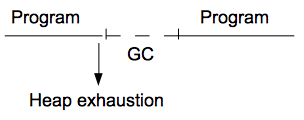
\includegraphics[scale=0.5]{stoptheworld.png}
\caption{Stop the world Garbage Collector \label{fig:stoptheworld}}
\end{figure}
Concurrent garbage collectors interleave the garbage collector as one or more thread along with the user program. Since, the garbage collector runs concurrently, a virtual lock needs to be used on the heap memory to avoid clashes between the garbage collector and the user program. They provide reduced latency but with a trade-off of bad throughput.
\begin{figure}[h]
\centering
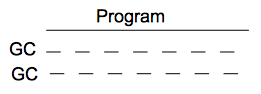
\includegraphics[scale=0.5]{concurrent.png}
\caption{Concurrent Garbage Collector\label{fig:concurrent}}
\end{figure}



\subsection{Serial vs. Parallel}
Serial garbage collectors execute only a single thread of the garbage collector program. However, a parallel garbage collector on the other hand, runs many garbage collector threads in parallel. Figure~\ref{fig:parallel} shows an embarrassing parallel program and Figure~\ref{fig:serial} shows an embarrassingly (inherently) sequential program. \\
\begin{figure}[h]
\centering
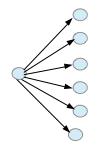
\includegraphics{embarrassinglyParallel.png}
\caption{Embarrassingly parallel program\label{fig:parallel}}
\end{figure}
\begin{figure}[h]
\centering
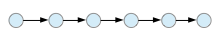
\includegraphics{embarrassinglySequential.png}
\caption{Embarrassingly sequential program\label{fig:serial}}
\end{figure}
\subsection{Non-moving/Non-relocating vs. Compacting}
Bump-pointer allocation is fast and the garbage collector is invoked only when we need more memory for allocation. Over time, the heap will get fragmented. Fragmentation is given by Equation~\ref{eq:frag}. So as to defragment the memory, the garbage collector identifies all pointers to memory and moves them to adjacent blocks. This is referred to as \textit{compaction}. A GC Map which contains the pointers of all objects can be obtained from the compiler for compaction.
\begin{equation}\label{eq:frag}
fragmentation = \frac{\text{Amount of heap allocated}}{\text{Amount of heap in use}}
\end{equation}
\begin{figure}[h]
\centering
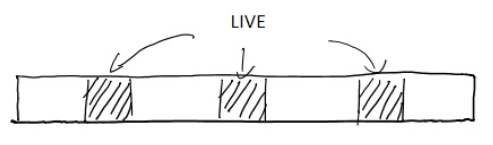
\includegraphics[scale=0.5]{fragmentation}
\caption{Fragmentation \label{fig:fragmentation}}
\end{figure}


\section{Incremental Garbage Collector}
Garbage collection is done in little bits incrementally. For example, the garbage collector can perform marking on a portion instead of marking the whole program.


\section{Generational Garbage Collector}
Generational garbage collector (also known as Partial Garbage Collector) is based on the generational hypothesis. The generational hypothesis states that most objects in a program die young - referred to as object mortality. In generational garbage collector, there are 2 heaps - $nursery$ and $old$. The garbage collector keeps track of the pointers in $old$ to $nursery$ in a "remembered set". During garbage collection, only the globals, stacks, "remembered set" and $nursery$ are scanned and memory is reclaimed from the $nursery$ (referred to as Minor Collection). Any data that wasn't reclaimed in the $nursery$ is copied to $old$ and all pointers are updated. $old$ is scanned and reclaimed once in a while (and this is referred to as Major Collection). Similarly, many different generation levels can exist in a generational garbage collector. Some collectors also have the $oldest$ generation referred to as $immortal$ because objects that are moved to this level are never reclaimed for the entirety of the program. Figure~\ref{fig:generational} shows generational garbage collector.
\begin{figure}[h]
\centering
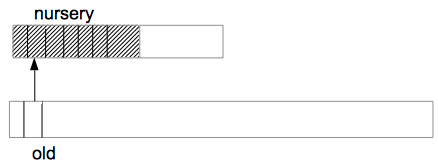
\includegraphics[scale=0.5]{generational}
\caption{Generational Garbage Collector \label{fig:generational}}
\end{figure}
\section{Semi-space Garbage Collector}
In a semi-space garbage collector, the heap is divided into 2 - $from$ and $to$. This requires 2X memory. Memory is allocated only from the $from$ heap. Once the $from$ heap is full, the garbage collector copies compactly data from the $from$ heap to the $to$ heap. All pointers are updated and forwarding pointers are left for memory in the $from$ heap. Now the $from$ heap becomes the $to$ heap and vice versa. Figure~\ref{fig:semispace} shows how semi-space garbage collectors work.
\begin{figure}[h]
\centering
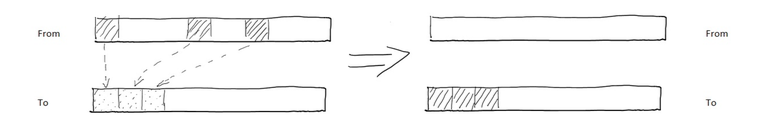
\includegraphics[scale=0.5]{semispace}
\caption{Semi-space Garbage Collector \label{fig:semispace}}
\end{figure}
\section{Thrashing and Locality}
Thrashing is an undesirable situation that occurs due to a constant state of paging, where data is swapped between memory and disk. Thrashing causes high degradation of performance.\\

There are 2 types of locality depending on how you access data in space and time:
\begin{enumerate}
\item Temporal Locality - refers to the reuse of same data within a small amount of time. Data that is most recently used has a higher probability of being used again.
\item Spatial Locality - refers to the idea that you are very likely to access neighboring locations in the very recent future when you access some data location.
\end{enumerate}
Caches use the idea of locality and help reduce latency. Garbage collectors generally have bad locality as they are very random in the memory locations they access.
\end{document}
